\section{Background}\label{chapter.background}
\thispagestyle{plain}
Before moving onto the technical substance of this thesis, acquiring a theoretical basis on the subject of this thesis will be beneficial. This chapter introduces software testing and explains a number of key concepts that are relevant to this thesis. Further, it presents constraint programming and optimization of test case scheduling as well as some previous work related to this thesis.

%%% SUBSECTION: Software Testing %%%
% Include something about gui testing. Check ASTvol3 (?)
\subsection{Software Testing}
\unsure[inline]{Maybe the existing test process should be described in this section as well, to give more context?}

A fundamental understanding of the concept of software testing is a useful prerequisite in order to understand the context of this thesis. Consequently, this section offers a short introduction to software testing. Since this is a large field, only relevant concepts and ideas will be presented. \comment{The testing strategy, process and technique used in this project will also be introduced here.} % and maybe test policy?

Software testing is the process of evaluating the quality of the application, system or component in question, commonly referred to as the test object or system under test (SUT). Software testing may involve any action oriented toward assessing the software with the goal of determining whether it meets the required results. \cite{[http://istqbexamcertification.com/what-is-a-software-testing/]}

Software is developed by human beings, who can make errors (mistakes). These errors may cause defects (faults, bugs) in the source code. Executing defected code can lead to failure in the program  \cite{http://www.istqb.org/downloads/send/2-foundation-level-documents/3-foundation-level-syllabus-2011.html}. One of the purposes of software testing is to examine the test object with the intent of revealing such defects. Other objectives include to measure and ensure quality, and to provide confidence in the product \cite[pp. 8]{SoftwareTestingFoundations}
%[The severity of a software defect can range from small and unimportant to largely expensive or even dangerous.]

%Software is developed by human, and humans are fallible. It is therefore sensible to presume that software may also have mistakes. The severity of a software defect can range from small and unimportant to largely expensive or dangerous. Releasing low-quality or faulty software may have critical consequences for businesses. 
\begin{figure}[h]
    \centering
    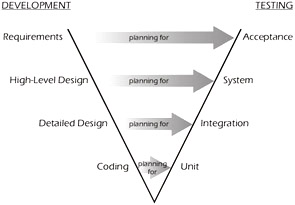
\includegraphics{figures/fig131_02}
    \caption{V-model \cite{http://flylib.com/books/en/2.174.1.22/1/} (Quality must be improved)}
    \label{fig.v-model}
\end{figure}

\subsubsection{The V-Model}

\noindent The \emph{V-model} plays an important role from the viewpoint of software testing. The central idea behind the model is to illustrate how each development task have a corresponding testing task of equal importance. This is symbolized by the two branches of the letter "V" in the model. The development process is represented by the left branch which shows the system being gradually designed. The integration and testing process is represented by the right branch, which shows how elements are progressively being assembled to form subsystems, and then tested \cite{SoftwareTestingFoundations}.

Depending on literature source, the V-model is used in different versions, covering varying amounts of detail and levels. The levels of the V-model shown in Figure \ref{fig.v-model} are explained below:

\begin{Description}
    \setlength{\itemsep}{1pt}
    \setlength{\parskip}{4pt}
    \setlength{\parsep}{0pt}
    \item[\betterfakesc{Requirements} $\Leftrightarrow$ \betterfakesc{Acceptance Test}]\hfill\\
    The requirements are gathered, specified and approved. Acceptance tests check if the requirements as specified in the contract are met. This is the highest development and test level of Figure \ref{fig.v-model}.
    \item[\betterfakesc{High-Level Design} $\Leftrightarrow$ \betterfakesc{System Test}]\hfill\\
    The functional design of the system is covered here. System testing verifies if the system as a whole meets the specified requirements.
    \item[\betterfakesc{Detailed Design} $\Leftrightarrow$ \betterfakesc{Integration Test}]\hfill\\
    Detailed design covers technical system design and component specification. Integration testing correspondingly verifies that the different components work together as specified.
    \item[\betterfakesc{Coding} $\Leftrightarrow$ \betterfakesc{Unit Test}]\hfill\\
    The specified components (modules, units, classes) are implemented. Component testing and unit testing verifies that system components perform as specified by testing them in isolation. This is the lowest development and test level of Figure \ref{fig.v-model}.
\end{Description}

\noindent \toolname \space is a tool for high-level test execution, that can be applied to the two highest test levels of the V-model; acceptance testing and system testing.


\subsubsection{Black-Box and White-Box Testing}
\noindent Software testing is divided into \emph{black-box} and \emph{white-box} testing. White-box testing is based on analysis of the internal system structure, and requires knowledge of the source code. In black-box testing, the test object is seen as black box, whose behavior is watched from the outside. The inner structure of the system is either not known or not considered. Test cases are determined from the specifications of the system. Black-box testing is predominantly used for higher levels of testing.

\toolname \space performs tests by using Selenium to automate web browsers. It executes functional UI tests on full system builds, and run without access or consideration to the source code and the internal system structure. The test method covered by \toolname \space is therefore black-box testing.

\comment{
    [CI - \url{http://stackoverflow.com/questions/17719385/how-to-make-jenkins-run-selenium-webdriver-testng-java-tests-automatically-on-de}]
}

%[http://istqbexamcertification.com/why-is-testing-necessary/]
% V-model should be here
% Maybe something about GUI testing? UI tests
% And something about cost of a bug/defect increasing rapidly as time goes by
%\\\\
%%% SUBSECTION: Generic Types of Testing %%%
%\subsubsection{Generic Types of Testing}
%\noindent
%\noindent

\comment{

    \subsubsection{Functional and Non-Functional Testing}
        \comment{
            \textsc{test2} % this should work
            {\scshape nå, då} % this should work
        }
    According to \cite{SoftwareTestingFoundations}, \emph{functional testing} seeks to validate that the test object behaves as specified in the functional requirements, which describes what the system should be able to do. A functional test is used to validate a particular feature for correctness. \emph{Non-functional testing} is aimed at testing the object for its non-functional requirements, that is to say the attributes of the functional behavior or the attributes of the system as a whole.
}

\comment{
\begin{Description}
    \item [Functional testing] seeks to validate that the test object behaves as specified in the functional requirements, which describes \emph{what} the system should be able to do. A functionality test is used to validate a particular feature for correctness.
    \item [Non-functional testing] is aimed at testing the object for its non-functional requirements, that is to say the attributes of the functional behavior or the attributes of the system as a whole.
    \comment{
        \item [Testing of software structure] involves the use of information about the internal code structure or architecture of the test object.
        \item [Testing related to changes] are conducted after changes has been implemented in the software.
    }
\end{Description}
}

\noindent

%\\\\
%%% SUBSUBSECTION: Methods of Testing %%%
%\subsubsection{Methods of Testing}
%\noindent

\comment{
\unsure[inline]{Maybe remove the two paragraphs below about static/dynamic testing as it is super boring and not really that relevant? At least not necessary in order to understand anything about this thesis, really...}
}

\comment{
    Further, \cite{SoftwareTestingFoundations} divides software testing methods into two categories; static and dynamic testing. Static testing is the testing of a component or system at specification or implementation level, and is conducted without executing the software, through forms of analysis such as document inspection.
    
    Contrary to static testing, dynamic testing explicitly involves the execution of the test object. An advantage to this method is that the actual program is executed either in its real environment or in an environment close to the real environment. This means that in addition to testing the design and code, elements such as the compiler, the libraries, the operating system and so on are also tested \cite{heinsBok}. Dynamic testing is the method addressed in this project.
}
%\\\\
%\noindent
%%% SUBSUBSECTION: Test Automation %%%
%\subsubsection{Test Automation}\label{subsubsection.test_automation}
\subsubsection{Test Automation}
As opposed to performing software tests manually, test automation is the practice of writing scripts that conduct tests when executed. Automation can be applied to tests at any level. Tests that exist at a low level, such as unit and component tests, generally run fast and are durable since they are isolated from changes in other parts of the system. These tests may be executed frequently. As we move up to the integration level, the tests does not run as fast, and become less durable since they are dependant on multiple components working together in subsystems. The tests at the highest levels, which includes system and acceptance testing, is concerned with testing the system at the perspective of the end user. These tests require the system to work as a whole, and thus generally run slower and are more brittle.

\cite{PLURALSIGHT lecture: Automated Testing: End To End}


User Interface tests are generally the fewest in number, as they are slower to run and more brittle.

Automated tests shouldn't be a complete replacement for manual human testing.

\comment{ [What should be automated? What can't be obtained through automated testing?]} While automated tests may run quickly and effectively, can be cost-effective and are useful for repeating tests the same way repeatedly, the natural exploration that occurs when humans perform manual testing does not happen through executing automated test scripts. Writing and maintaining test scripts are time consuming, so it is important to only use resources on automating test cases of value. Tests and tasks that would be error prone if done manually are typical subjects for automation \cite{ASTvol3}. This includes regression testing, which is the testing of a previously tested object after changes are made in the software or its environment, and is done to detect any new defects that has been introduced after the changes \cite{SoftwareTestingFoundations}. Test automation should not replace manual testing as a whole; the two should complement each other through a combination of adequate amounts of both manual and automated testing.

There are some pitfalls that one should be aware of upon entering the area of test automation. It is not uncommon that companies generally have unrealistic expectations of test automation, and expect that including test automation in a software project guarantees instant success, which is not the case. Another typical mistake is believing that test automation requires less time and resources than it actually does \cite{ASTvol3}.

However, the benefits of applying test automation to software projects are many. When considering the benefits of automated testing, these are compared to the duration, effort, or coverage that would have alternatively been obtained through manual testing. While simultaneously saving time, reducing effort and providing better coverage and thus lower risk, additional benefits to choosing test automation may include better predictability of test execution time. Some types of testing are hard, impractical, or even impossible to conduct manually, at least not in a meaningful way. These types of testing include performance, stress, load, and reliability testing, which are all areas that can be tested with the right automation in place, and in turn reduce the risk \cite{ASTvol3}.

\comment{
    IEEE/ISO Standard
    ISTQB Websiden (terminologi etc.)
    Software Testing boken
    
    * Se på test nivåer - må forklare på hvilket nivå disse testene utføres.
    * Se på test tilnæringer - f.ekx. black, white, grey box testing eller context driven testing. Finnes og andre. Sjekk litteratur. Du driver med black/grey box testing hvis man ser det utfra det perspektivet.
    * Se på forskjellige test teknikker/metoder - statisk testing, dynamisk testing, funksjonell vs. icke-funksjonell testing etc.
    * Teststrategi, -policy og -prosess -- input fra Alitbox. Spør hva de har for dokumentasjon rundt dette. Ellers finnes dette i IEEE standard. Fornuftig å skrive at du har valgt en strategi, policy og prosess for tid arbeid. Kanskje strategi og prosess er spesielt viktig. Policy er kanskje ikke nødvendig da det ofte er veldig orgranisasjonsspesifikkt.
    
    
    test strategy-A test strategy is an outline that describes the testing approach of the software development cycle.
    test levels - systemtest, integrasjonstest, akseptansetest osv.
    test metode/teknikk - black, white box testing
    test type - 
    
    non-functional testing - the way the system operates.
    functional testing - what the system does
    
    Functional testing is a quality assurance (QA) process[1] and a type of black-box testing 
}

%%% SUBSECTION: Constraint Programming and Optimization %%%
\subsection{Constrained Optimization}
\todo[inline]{Write this section}

%%% SUBSECTION: Related Work %%%
\subsection{Related Work}
Some work has previously been done on the subject of test case scheduling and automation of UI tests for web applications. This section presents the scheduling method \emph{TC-Sched} and the automated testing platform \emph{Sauce Labs}.

\subsubsection{TC-Sched}
TC-Sched is a time-aware method for minimizing the execution time of test cases within a distributed system with resource constraints. The method was proposed by Mossige, Gotlieb, Meling, and Carlsson in \cite{tcsched}. The authors consider the following in their paper:


\begin{itemize}
    \item A set of test cases $\cmsy{T} = \{t_{1}, \dots, t_{n}\}$ along with a function $d : \cmsy{T} \longrightarrow \mathbb{N}$ that gives each test case a duration $d_{i}$
    \item A set of global resources $\cmsy{G} = \{g_{1}, \dots, g_{o}\}$ along with a function $g : \cmsy{T} \longrightarrow \cmsy{G}$ that describes which resources are used by each test case
    \item A set of machines $\cmsy{M} = \{m_{1}, \dots, m_{m}\}$ along with a function $f : \cmsy{T} \longrightarrow \cmsy{M}$ which assigns a subset on machines to each test case on which the test case can be executed
\end{itemize}

\noindent They further define the \emph{optimal test case scheduling} (OTS) as the optimization problem $(\cmsy{T}, \cmsy{G}, \cmsy{M}, d, g, f)$ of finding an execution ordering and assignment of all test cases to machines, such that each test case is executed once, no global resource is used by two test cases at the same time, and the overall test execution time, $T_{t}$, is minimized. $T_{t}$ is the time it takes to solve the scheduling problem, $T_{s}$, plus the time it takes to execute the schedule, $C$*, $T_{t} = T_{s} + C$*.

As established in the bullet list above, TC-Sched addresses situations in which some operations may require exclusive access to one or more \emph{global resources}, such that only one test case can access each resource at a given time. To include the aspect of global resources in this project would have been redundant since there are no such global resources involved. Apart from that, TC-Sched is a closely related scheduling method that has been of inspiration. The implementation of the scheduling algorithm used in this project will be described in Chapter \ref{chapter.implementation}.

\unsure[inline]{Brief description of their algorithm, maybe? Maybe a figure? Or maybe have that in implementation chapter? Or maybe not?}

\subsubsection{Sauce Labs}
Cloud testing services use cloud computing environments as a means of simulating real-life user traffic. Sauce Labs is a cloud-hosted platform for automated testing of web and mobile applications. One of the founders, Jason Huggins, were also the original creator of Selenium, which will be introduced in Section \ref{subsec.selenium}.

Sauce Labs bear some similarities and some dissimilarities with the design of \toolname. They both support automated testing of web applications using Selenium and allow remote testing in distributed environments through the use of Selenium Grid (see Subsection \ref{subsubsec.seleniumGrid}). However, whereas Sauce Labs perform test execution solely on virtual machines that are created prior to each test run, and then destroyed immediately after, \toolname \space requires the use of real, physical machines or devices, or customized virtual machines or devices running on said physical machines or devices, so that the user remains in complete control at all times. Additionally, Sauce Labs executes tests in their own data centers contained in an remote location, with their own environments, while \toolname \space tests the test object locally and in its intended environment. Further, Sauce Labs do not automatically create issues in the issue tracker. Sauce Labs is a paid service for which customers pay to gain access to using a limited number of concurrent virtual machines for a limited amount of time each month. The optimization algorithm in this project also distinguishes the two projects even further. % SOURCE!

\comment{
    - TC-sched etc
    - Saucelabs:
        + Similarities: Uses Selenium Grid and Selenium WebDriver(?), supports distributed testing and all other benefits of Selenium+Selenium Grid.
        - Dissimilarities: Runs tests on virtual machines in the cloud; _not_ in a distinguished suitable environment, and _not_ on real, physical machines/devices that we are in complete control over. Does not create tasks in the issue tracker. Maybe: Runs all tests in parallell? And does not (?) provide a OTS/task scheduling algorithm. Costs money: pay a certain amount for accessing a limited number of VMs a limited number of minutes each month. In this solution, you can use real-life physical company owned devices and machines or customized virtual machines as much as desired at anytime.
}